\begin{figure}[!htb]
\begin{center}
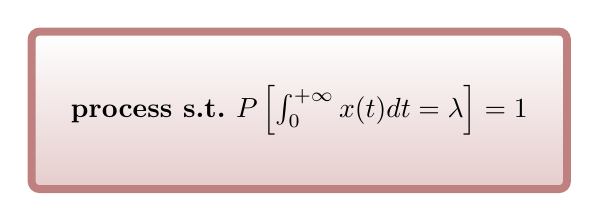
\begin{tikzpicture}
[
	xscale	= 1,	% to scale horizontally everything but the text
	yscale	= 1,	% to scale vertically everything but the text
]

\node
(nProcessNode)							% name of the node
[										% properties of the node:
	shape			= rectangle,		% shape
	rounded corners	= 0.1cm,			% roundness of the corners
	minimum height	= 2cm,				% | minimum size
	minimum width	= 6cm,				% |
	line width		= 0.1cm,			% thickness of the border
	draw			= red!50!black!50,	% colour of the border
	top color		= white,			% | filling colors
	bottom color	= red!50!black!20,	% |
	font			= \bfseries,		% used font
	inner xsep		= 0.5cm,			% minimum distance btw text and borders along x dimension
	inner ysep		= 0.5cm				% minimum distance btw text and borders along y dimension
]
{process s.t.\ $\mathbb{P} \left[ \int_{0}^{+\infty} x(t) dt = \lambda \right] = 1$}; % DON'T FORGET THE SEMICOLON!!

\end{tikzpicture}
\end{center}
\end{figure}
